
% This LaTeX was auto-generated from MATLAB code.
% To make changes, update the MATLAB code and republish this document.

\documentclass{article}
\usepackage{graphicx}
\usepackage{color}

\sloppy
\definecolor{lightgray}{gray}{0.5}
\setlength{\parindent}{0pt}

\begin{document}

    
    
\subsection*{Contents}

\begin{itemize}
\setlength{\itemsep}{-1ex}
   \item HW1, Q 3.10
   \item Parameters
   \item A, B, C, D Matrices
   \item Simulation
\end{itemize}
\begin{verbatim}
clc; clear all; close all; format compact

% Jack Vranicar
% jjv20@fsu.edu
\end{verbatim}


\subsection*{HW1, Q 3.10}



\subsection*{Parameters}

\begin{verbatim}
m_3 = 1; % kg
m_2 = 2; %kg
m_1 = 1; %kg

f_v3 = 1; % N*s/m
f_v2 = 1; % N*s/m
f_v1 = 1; % N*s/m

k_2 = 1; % N/m
k_1 = 1; % N/m
\end{verbatim}


\subsection*{A, B, C, D Matrices}

\begin{verbatim}
A = [
    0 , 1 , 0 , 0 , 0 , 0;
    -k_2/m_1 , (-f_v3 - f_v2)/(m_2) , 0 , (f_v2)/(m_2) , (k_2)/(m_2),...
    (f_v3)/(m_2);
    0 , 0 , 0 , 1 , 0 , 0;
    0 , (f_v2)/(m_2) , (k_1)/(m_2) , (-f_v2 - f_v1)/(m_2) , (k_1)/(m_2),...
    (f_v2)/(m_2);
    0 , 0 , 0 , 0 , 0 , 1;
    (k_2)/(m_3) , (f_v3)/(m_3) , (-k_1)/(m_3) , (f_v1)/(m_3),...
    (k_1 - k_2)/(m_3) , (-f_v3 - f_v1)/(m_3);
    ];

B = [

0;
0;
0;
0;
0;
(1)/(m_3);

];

C = [

1 , 0 , 0 , 0 , 0 , 0 ;
0 , 0 , 1 , 0 , 0 , 0 ;
0 , 0 , 0 , 0 , 1 , 0 ;


];

D = [
    0;
    0;
    0;
];
\end{verbatim}


\subsection*{Simulation}

\begin{verbatim}
T = ss(A, B, C, D);

Z = initial(T, [1 0 0 0 0 0], 10);
times = linspace(0, 10, numel(Z(:,1)));

figure("WindowState", "maximized")
    hold on
    set(gca,'FontSize',20);
    subplot(3, 1 ,1)
    plot(times, Z(:,1))
    set(gca,'FontSize',20);
    title("Problem 3.10")
    ylabel("x_1")
    subplot(3, 1, 2)
    plot(times, Z(:,2))
    set(gca,'FontSize',20);
    ylabel("x_2")
    subplot(3, 1, 3)
    plot(times, Z(:,3))
    set(gca,'FontSize',20);
    ylabel("x_3")
    xlabel("Time (s)")
    hold off
\end{verbatim}

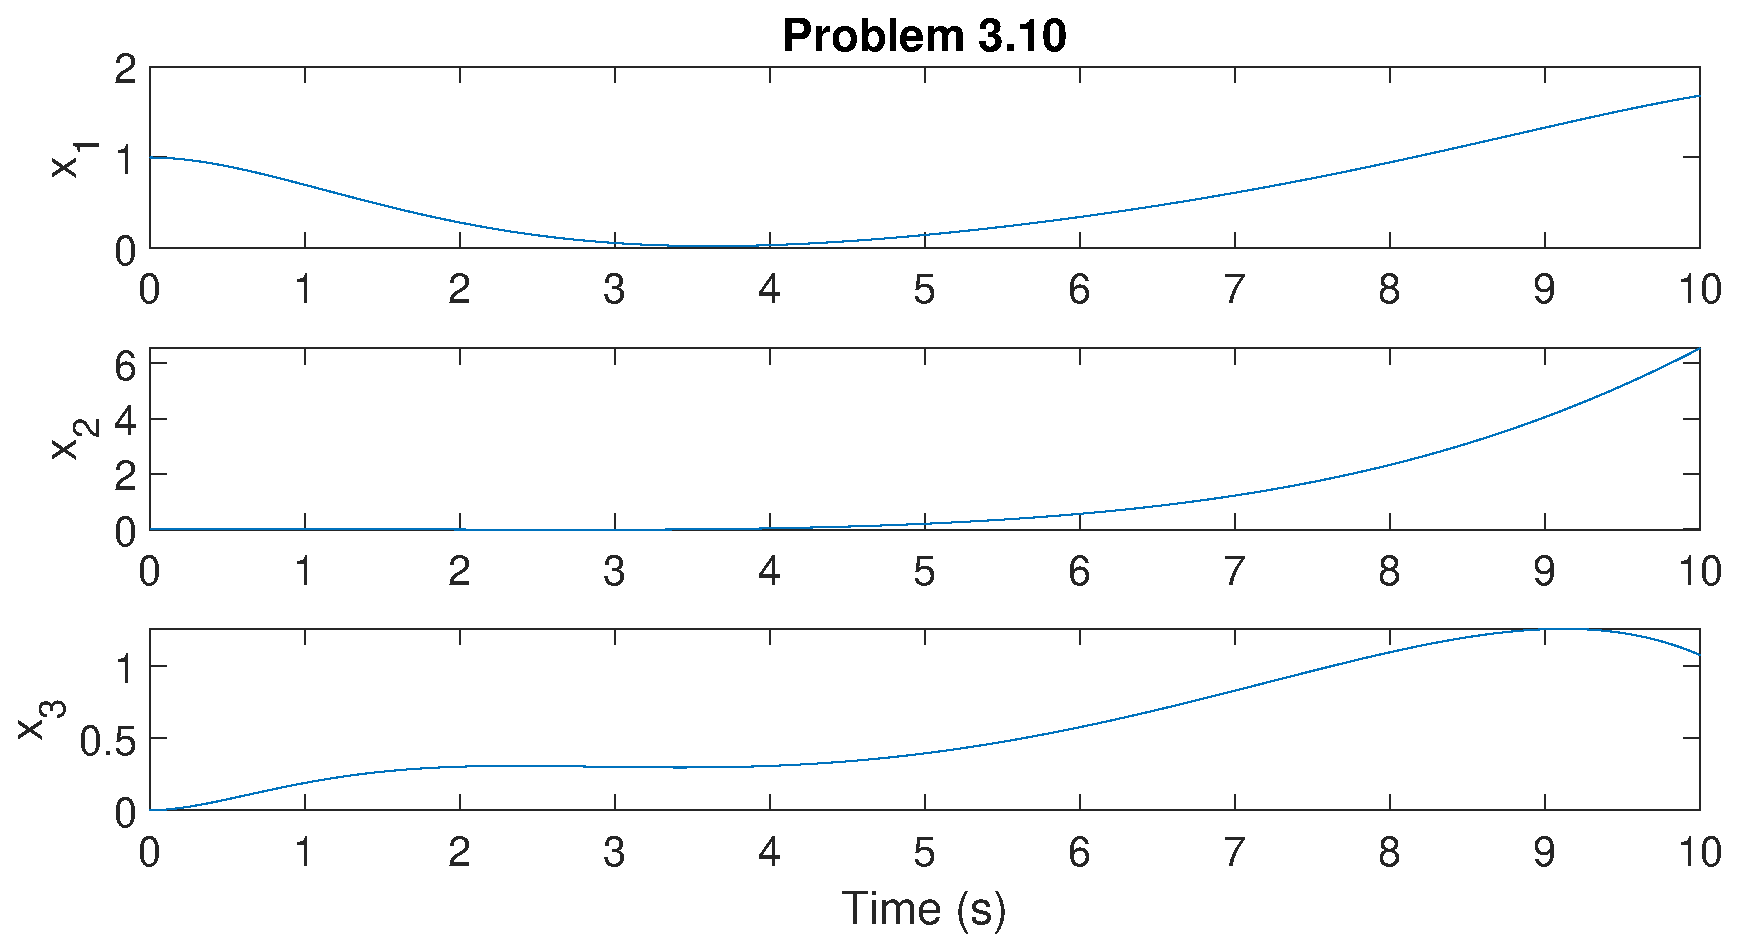
\includegraphics [width=4in]{q3_10_01.eps}



\end{document}

